\documentclass[12pt,twocolumn]{article}
\usepackage[T1]{fontenc}
\usepackage{graphicx}
\usepackage{tabularx}
\usepackage{amsmath,amsthm,amssymb}
%\usepackage{esvect}
\usepackage[left=1cm,right=1cm,top=1.75cm,bottom=2cm]{geometry}
%\renewcommand*{\familydefault}{\sfdefault}
\title{\vspace{-2.5em}Convection in 2 Dimensions}
\author{Christopher Pattison}
\date{}
\begin{document}
\maketitle
\section*{Derivation}
Pure convection can be modeled by the conservation law \eqref{eq:conservlaw}.
\begin{equation}\label{eq:conservlaw}\nabla\cdot\rho\vec{u}C_PT = 0\end{equation}
In two dimensions, the equation is integrated over the volume and the divergence theorem applied \eqref{eq:fvm}.
Material properties, velocity, and grid spacing were assumed constant, resulting in equation \eqref{eq:discr}.

\begin{equation}\label{eq:fvm}\int_V \nabla\cdot\rho\vec{u}C_PT dydx = 0\end{equation}
\begin{equation}F=\rho\vec{u}C_P\end{equation}
\begin{equation}\label{eq:discr}(FT)_e\delta y - (FT)_w\delta y +
(FT)_n\delta x - (FT)_s\delta x\end{equation}

An interpolation scheme for $T$ is selected and a system solver applied.

\subsection*{Boundary Conditions}
The boundary conditions and properties are given by Equations (\ref{eq:uval}-\ref{eq:zeroflux}).
A pecularity of these boundary conditions is that Gauss-Seidel can solve the resulting system in a single sweep in certain directions.
\begin{equation}\label{eq:uval}\rho C_P u= \rho C_P v=\frac{\sqrt{2}}{2}\end{equation}
\begin{equation}\left.T\right|_{x=0} = 1;\hspace{1ex}\left.T\right|_{y=0} = 0\end{equation}
\begin{equation}\label{eq:zeroflux}\left.\frac{\partial T}{\partial y}\right|_{x=1} = \left.\frac{\partial T}{\partial y}\right|_{y=1} = 0\end{equation}
\section*{Deferred Correction}
In first-order upwinding, the value of $T$ at the face is assumed to be equal 
to the value of the upwind node. This unconditionally guarantees a positive coefficient,
but will result in artificial, ``cross'' diffusion if the flux is not perpendicular to the cell face.
This is due to the upwind node not being directly upwind.

Central differencing will not suffer from artificial diffusion, but will be unstable in pure convection problems as $P = \infty$ results in $a_P = 0$.
The accuracy of the solution can be increased by deferred correction \eqref{eq:defcorr},  which combines a low order scheme with a higher order scheme.

\begin{equation}\label{eq:defcorr}\Phi = \Phi_L + \beta (\Phi_H - \Phi_L)^{k-1}\end{equation}

Where $\Phi$ is a high ($H$) or low ($L$) order discretization. 
The blending factor $\beta$ determines how close the resulting solution will be to the high ($\beta = 1$) or low ($\beta = 0$) order solution.
The result of deferred correction is a non-linear source term \eqref{eq:source}.

\begin{equation}\label{eq:source}S = \beta (\Phi_H - \Phi_L)^{k-1}\end{equation}

Central differencing, while unusable without diffusion, is well suited as a higher order scheme to increase the accuracy of upwinded solutions.

\begin{figure}
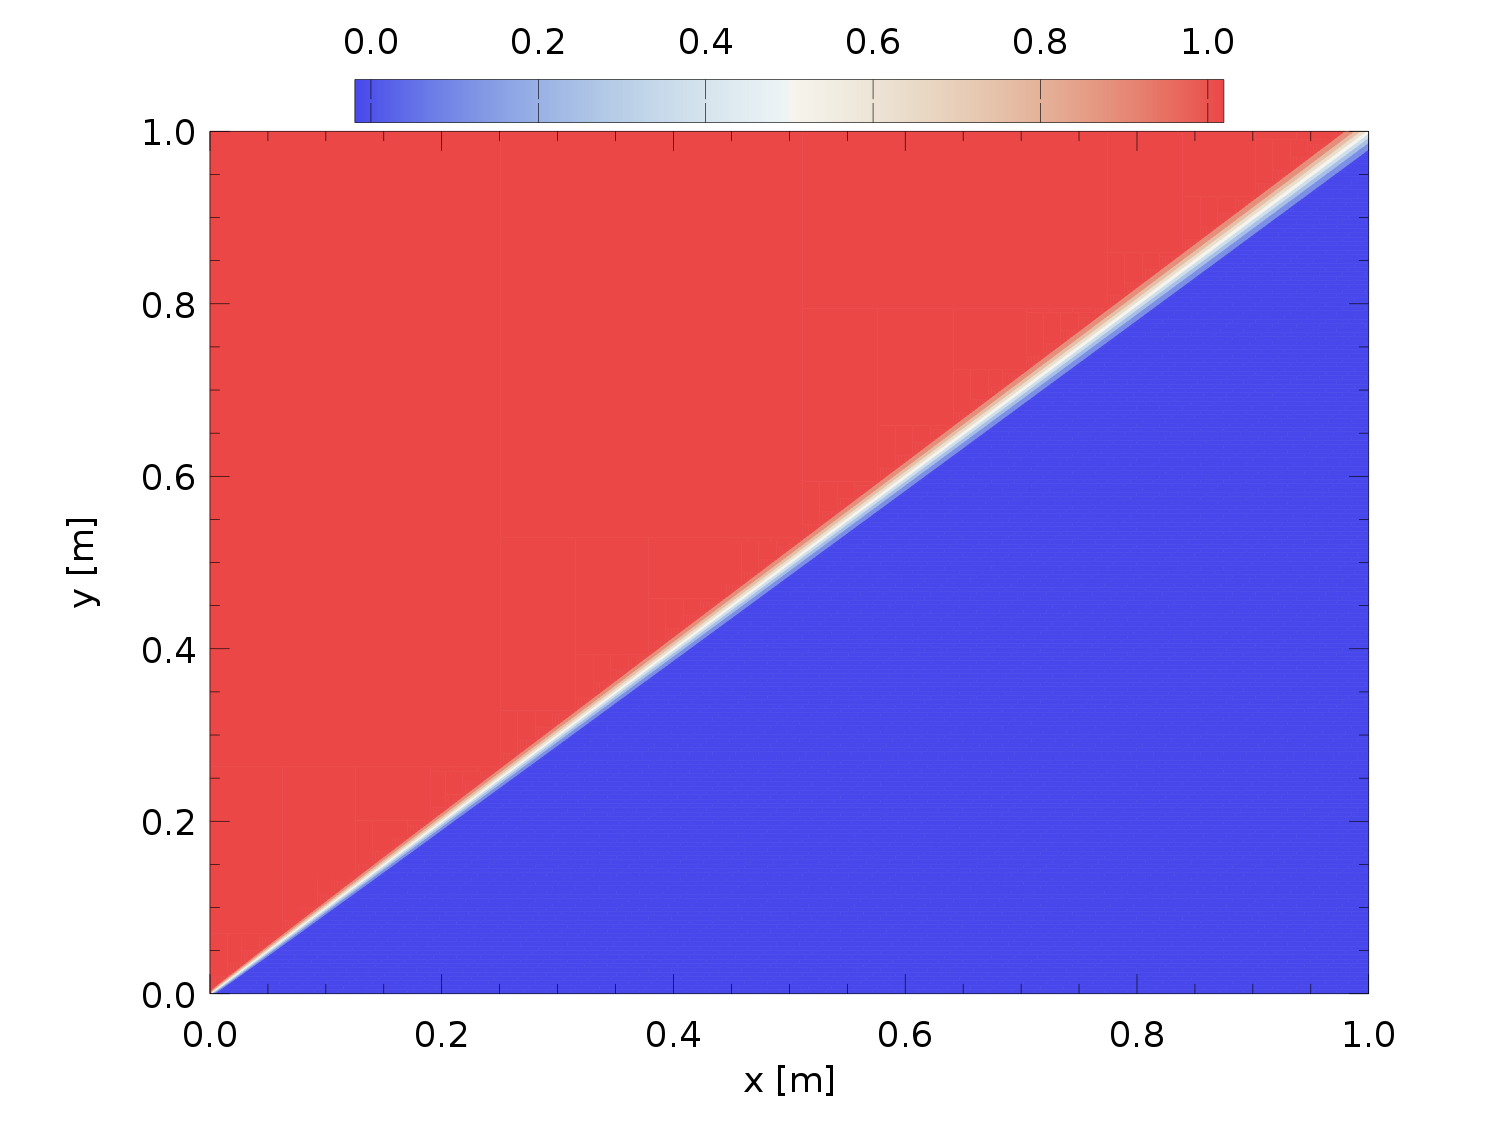
\includegraphics[width=\columnwidth]{plot/DcSolution.png}
\footnotesize{\caption{Deferred Correction ($\beta$ = .95)}\label{fig:solution}}
\end{figure}

\section*{Solution}
The true solution is represented by equation \eqref{eq:solution}.
Notably, the solution has no derivatives and is discontinuous.
\begin{equation}\label{eq:solution}T =
\begin{cases}
1 & y > x \\
0 & y \leq x
\end{cases}
 \end{equation}
The solution obtained with first-order upwinding was extremely diffusive as compared to the differed correction solution by fig. \ref{fig:diff}, the plot of equation \eqref{eq:norm}.
\begin{equation}\label{eq:norm}\delta = \frac{(T_{DC} - T_{UPW})^2}{\langle(T_{DC} - T_{UPW})^2\rangle}\end{equation}
As $\beta$ increased, the cross diffusion reduced, although $\beta = 1$ diverges as expected since pure central differencing is unstable.

\begin{figure}
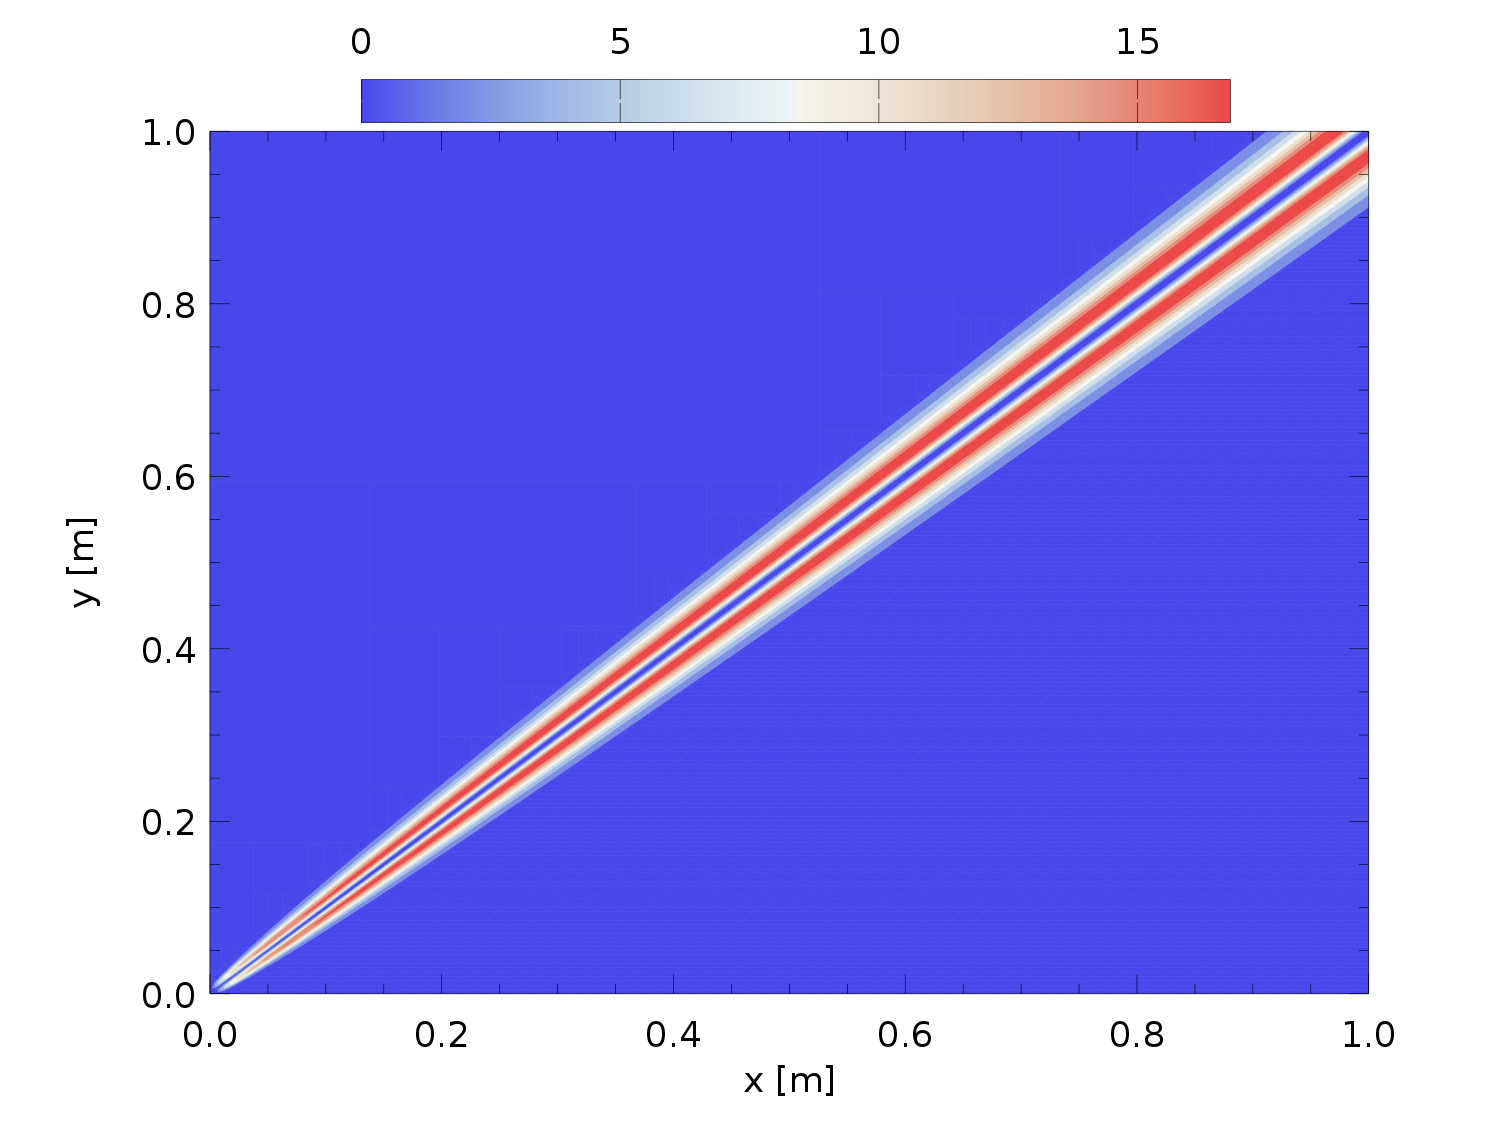
\includegraphics[width=\columnwidth]{plot/DcUpwDiff.png}
\footnotesize{\caption{Normalized Difference Squared}\label{fig:diff}}
\end{figure}

\section*{QUICK}
\begin{figure}
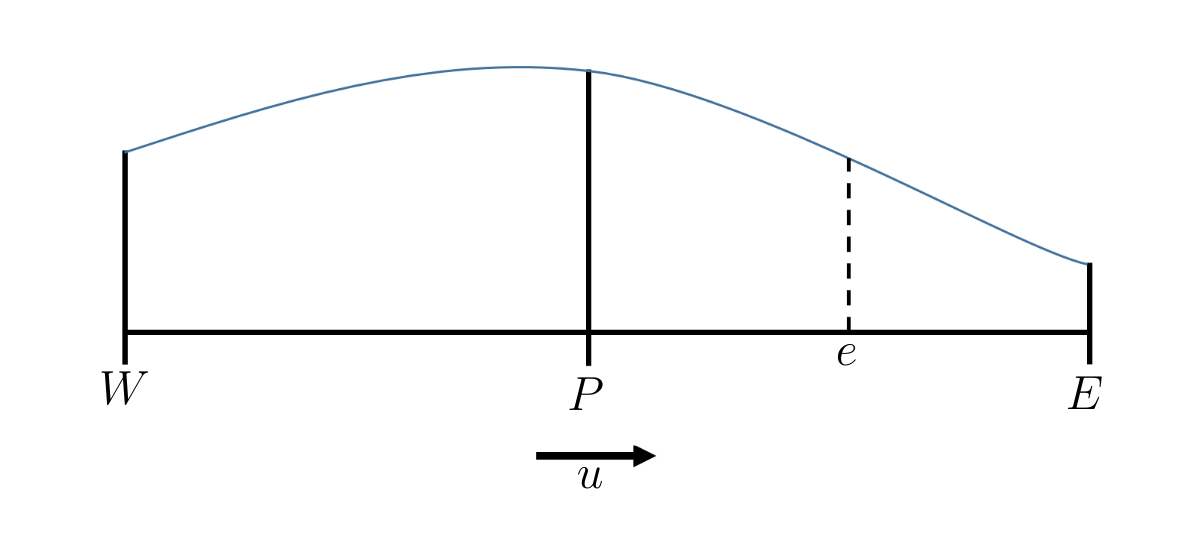
\includegraphics[width=\columnwidth]{plot/QUICK.png}
\footnotesize{\caption{QUICK interpolation}\label{fig:quick}}

\end{figure}
The QUICK scheme uses a quadratic polynomial to interpolate the value of $T$ at the cell face.
Two upwind nodes are used as well as a single downwind node.
While QUICK still suffers from cross diffusion, it is reduced considerably due to the high order of the scheme $O(h^3)$.
Fitting the polynomial results in equation \eqref{eq:quickinterp} for the value of $T_e$ with $u>0$.
\begin{equation}\label{eq:quickinterp}T_e = \frac{3}{8}T_E + \frac{3}{4}T_P - \frac{1}{8}T_W\end{equation}
A disadvantage of the scheme becomes apparent when the interpolations for $T_w$ and $T_s$ are considered.
Since a second upwind node is required, the computational stencil must be extended to include the $T_{WW}$ and $T_{SS}$ nodes.

Figure \ref{fig:quickslice} makes apparent that QUICK is prone to oscillations about slope discontinuities.
Another oddity is the overshooting of the true value of the solution.
Attempting to keep the overshoot from occurring by enforcing the boundary conditions in \eqref{eq:forcebounds} proved unsuccessful with nearly no change in the solution.
\begin{equation}\label{eq:forcebounds}\left.T\right|_{x=1} = 0;\hspace{1ex}\left.T\right|_{y=1} = 1\end{equation}
It is believed that the overshoot is due to the discontinuity in the true solution, because using QUICK as the high order discretization in deferred correction resulted in a reduction of the overshoot.
It is likely that QUICK could be used if upwinding was used to interpolate the value of cell faces immediately adjacent to the discontinuity where the solution has no derivatives.
\begin{figure}
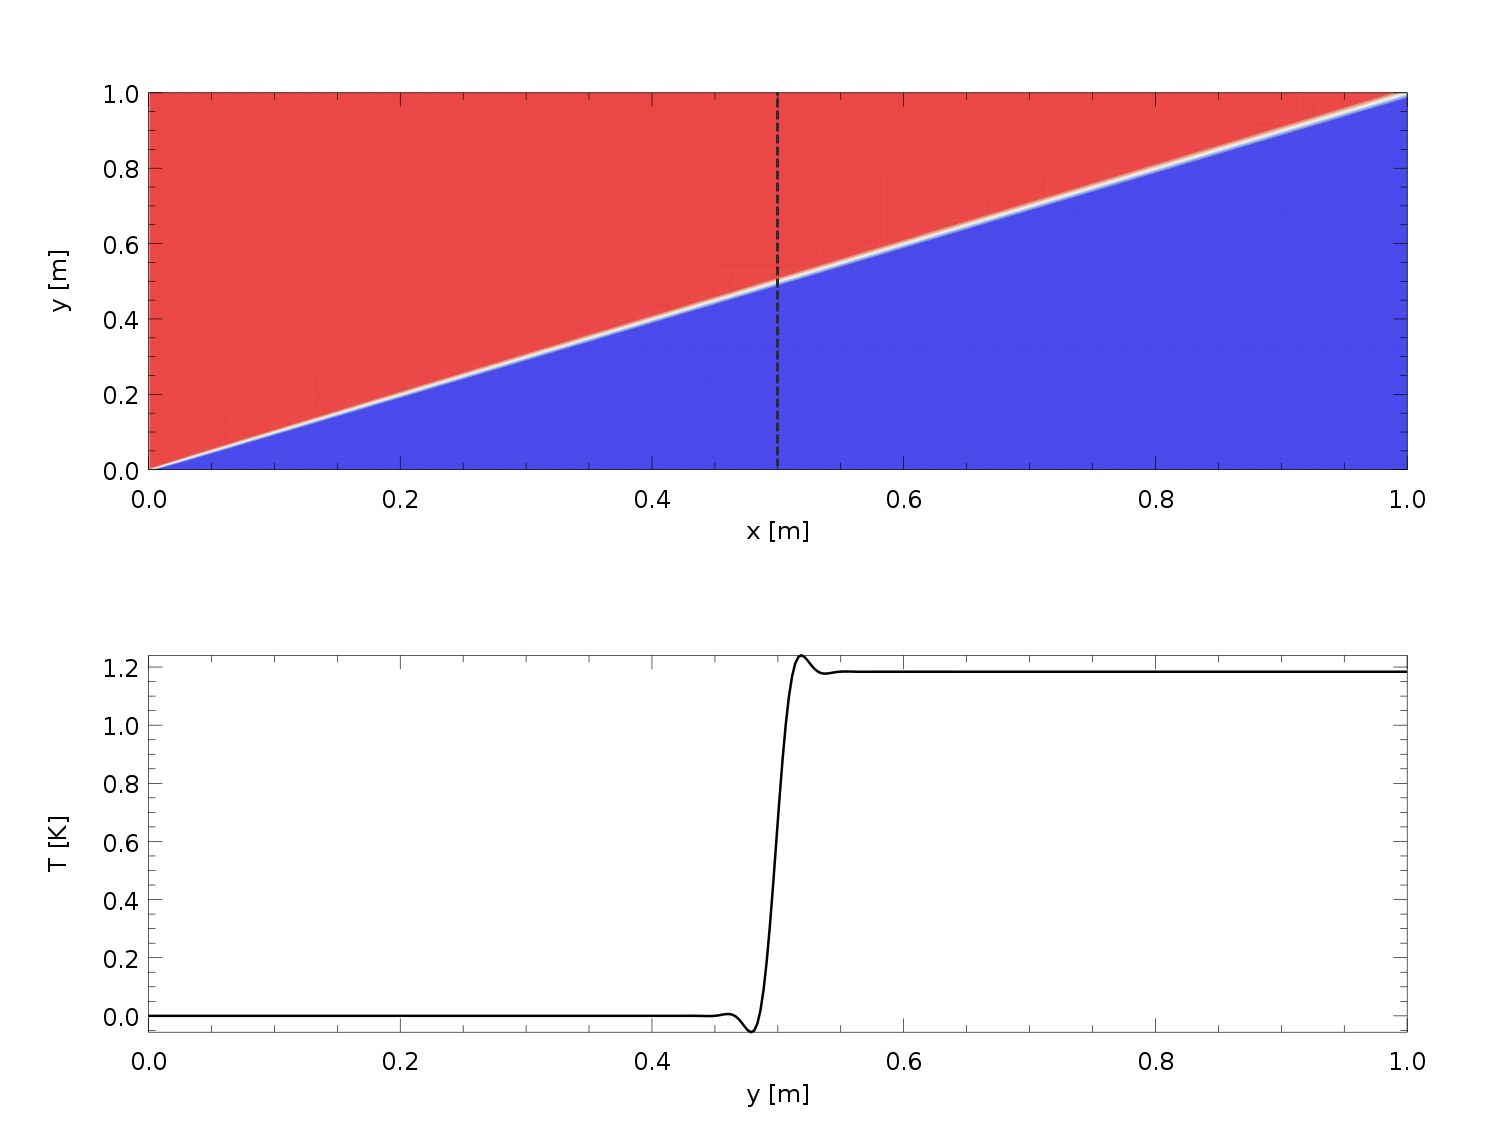
\includegraphics[width=\columnwidth]{plot/QuickSlice.png}
\footnotesize{\caption{Solution obtained with QUICK}\label{fig:quickslice}}
\end{figure}
\end{document}

